\section{Findings}
\label{sec:findings}


\subsection{Decrease and increase in accumulation precision}

The insufficient Tensor Core accumulation precision on the Hopper architecture has caused LLM training instability, as reported by \cite{deepseek-ai_deepseek-v3_2024}. We find that this issue also exists on the Ada Lovelace architecture. According to our bit-accurate reference model, the QMMA instructions of the Ada Lovelace architecture use the FDA or CoFDA algorithms with 13 fractional bits, the same as the QGMMA instructions of the Hopper architecture, which also use the FDA algorithm with 13 fractional bits (instead of 14 mantissa bits reported by \cite{deepseek-ai_deepseek-v3_2024}). In comparison, their TF32, FP16, and BF16 instructions use 24 (Ada Lovelace) or 25 (Hopper) fractional bits.

However, we find that NVIDIA has resolved this issue on its latest architectures (Blackwell and RTX Blackwell) by increasing the precision of the FP8 matrix multiplication instructions to 25 fractional bits, the same as the accumulation precision of the TF32, FP16, and BF16 instructions on both architectures. In addition, AMD uses 24 fractional bits for the FP8 instructions, as shown in the FDRDA and GFDRDA algorithms.

\textbf{Architectural insight.} In summary, most Tensor Core and Matrix Core instructions use at least 23 fractional bits, except for the FP8 instructions of the Ada Lovelace and Hopper architectures. Therefore, for future MMA designs, we suggest using at least 23 fractional bits (i.e., the number of mantissa bits of FP32). More bits are also beneficial to numerical accuracy.

\textbf{Software insight.} On the Hopper and Ada Lovelace architectures, we suggest that software developers should use the FP16 or BF16 instructions for FP8 matrix multiplication, sacrificing efficiency for higher precision.

\subsection{Limited dynamic range}

The subnormal flushing behavior of CDNA2 can impact DNN training stability, as reported by \cite{pytorch_developers_pytorch_2025}. We find that AMD has resolved this issue on the CDNA3 architecture by fully supporting subnormal numbers, as shown in the FDRDA, CoFDRDA, GFDRDA, and CoGFDRDA algorithms. However, we also note that intermediate products overflow to infinity when their absolute values exceed $2^{128}$. In comparison, on NVIDIA Tensor Cores, the intermediate products do not overflow, as shown in the FDA, CoFDA, and GDFS algorithms.

\textbf{Architectural insight.} In summary, except CDNA2 Matrix Core, all Tensor Cores and Matrix Cores support the dynamic range of FP32. For future MMA designs, we suggest fully supporting the dynamic range of FP32 including subnormal numbers to prevent the DNN training issue. Avoiding overflow in intermediate results is also beneficial.

\textbf{Software insight.} On the CDNA2 architecture, we suggest that software developers should scale or normalize the inputs of FP16 matrix multiplication to avoid subnormal numbers. Alternatively, sacrificing precision, software developers can use BF16 instructions for FP16 matrix multiplication, as suggested by \cite{pytorch_developers_pytorch_2025}.

\subsection{Asymmetric rounding on CDNA3}

We find that most Tensor Core and Matrix Core instructions use symmetric rounding modes such as rounding to zero (RZ) and rounding to nearest, ties to even (RNE). However, the TF32, FP16, and BF16 MFMA instructions of the CDNA3 architecture use the rounding down (RD) mode, which is asymmetric. Using the RD mode may introduce non-negligible numerical errors and numerical biases under certain circumstances, as shown below.

(a) Numerical error. We take CDNA3 FP16 MFMA instruction v\_mfma\_f32\_32x32x8\_f16 for example. To demonstrate the significance of the error, we set $a_0=a_1=b_0=2048$, $b_1=-2048$, $c=-0.000001$, and all other inputs to zero. During the computation, $c$ is rounded down to $-2^{-2}=-0.25$, as shown in Step 6 of FDRDA. Therefore, the computational result of $2048\times2048-2048\times2048-0.000001$ is $-0.25$, which greatly deviates from the real result $-0.000001$. The absolute error is $0.249999$. In comparison, using other instructions with RZ or RNE to compute $2048\times2048-2048\times2048-0.000001$ results in $0.0$, whose absolute error is only $0.000001$.

(b) Numerical bias. To demonstrate the numerical bias, we use MMA-Sim to simulate CDNA3 v\_mfma\_f32\_32x32x8\_f16 instruction and a hypothetical v\_mfma\_f32\_32x32x8\_f16\_rz instruction that uses RZ instead of RD. We generate random values from the standard normal distribution $N(0,1)$ for $C$, and the normal distribution $1000\times N(0, 1)$ for $A$ and $B$. Sending these inputs to MMA-Sim, we obtain the CDNA3 output $D_{RD}$ and the output of the hypothetical MMA $D_{RZ}$. We also compute the real result $D_{real}$ using FP64, and compute $\delta_{RD}=D_{RD}-D_{real}$ and $\delta_{RZ}=D_{RZ}-D_{real}$. As Figure \ref{fig:delta} shows, the distribution of $\delta_{RD}$ is biased to the negative direction while the distribution of $\delta_{RZ}$ is symmetric.

\begin{figure}[ht]
    \centering
    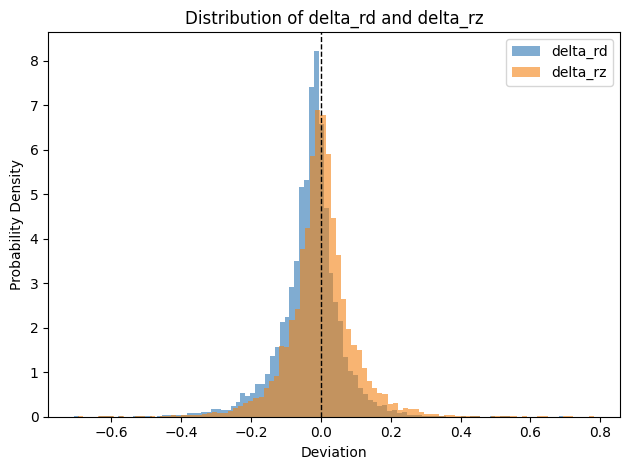
\includegraphics[width=1\linewidth]{figures/delta.png}
    \caption{Distributions of $\delta_{RD}$, numerical deviation of CDNA3 FP16 MFMA instruction that uses the rounding-down (RD) mode, and $\delta_{RZ}$, numerical deviation of a hypothetical FP16 MFMA instruction that uses the rounding-to-zero (RZ) mode.}
    \label{fig:delta}
\end{figure}

These phenomena occur when $A$ and $B$ contain large-magnitude numbers and the elements of $C$ are negative numbers with relatively small magnitudes. We note that AMD has added a patch to CDNA3 FP8 MFMA instructions. As shown in Step 8 of GFDRDA, there is an additional check for the exponent of $c$. If $e_c<e_{max}-25$, then $c$ is rounded to zero instead of rounded down. This patch avoids the cases above.

\textbf{Architectural insight.} We note that if the hardware uses two's complement encoding to store and compute intermediate sums, RD is the most natural choice for rounding because RD can be implemented by simply truncating the least significant bits in two's complement encoding. In addition, if hardware uses ones' complement or sign-magnitude encoding, RZ is the most natural choice because RZ can be implemented by simply truncating the least significant bits in these encodings. Because floating-point numbers are based on the sign-magnitude encoding, we suggest using sign-magnitude arithmetic as well and choosing RZ as the rounding mode.

\textbf{Software insight.} On the CDNA3 architecture, we suggest using Matrix Cores only for matrix multiplication by setting $C=0$, and using the general compute units for full FP32-precision matrix accumulation to mitigate this issue in the TF32, FP16, and BF16 instructions.
